% IEEE Design & Test (D&T) magazine feature submission.
% Magazine-style rewrite (~5,000 words), NOT a compression of the arXiv
% preprint: fresh prose throughout; the preprint is cited for depth.
% All numbers trace to docs/paper/PRESUBMISSION_DISCLOSURES.md.
\documentclass[conference]{IEEEtran}
\IEEEoverridecommandlockouts
\usepackage{cite}
\usepackage{amsmath,amssymb}
\usepackage{xcolor}
\usepackage{booktabs}
\usepackage{threeparttable}
\usepackage{tikz}
\usetikzlibrary{positioning,arrows.meta,calc}
\usepackage{url}

\newcommand{\code}[1]{\texttt{\detokenize{#1}}}

\begin{document}

\title{When the Golden Model Is Wrong Too: Industrial-Grade
	Verification for an Open-Source GPGPU}

\author{\IEEEauthorblockN{Samuel Moussa\IEEEauthorrefmark{1},
		Steven Ibrahim\IEEEauthorrefmark{1},
		Ahmad Sudky\IEEEauthorrefmark{1},\\
		Ahmad Fawzy\IEEEauthorrefmark{1},
		Abanoub Nabil\IEEEauthorrefmark{1},
		Alhassan Sayed\IEEEauthorrefmark{1},\\
		Hossam Hassan\IEEEauthorrefmark{2}, and
		Hyung-Min Yoon\IEEEauthorrefmark{3}}
	\IEEEauthorblockA{\IEEEauthorrefmark{1}Department of Electronics and
		Communications Engineering,\\
		Faculty of Engineering, Minia University, Egypt\\
		\IEEEauthorrefmark{2}Independent Researcher, South Korea \quad
		\IEEEauthorrefmark{3}Siliconarts, Inc., South Korea\\
		Corresponding author: samuelmoussa64@gmail.com}}

\maketitle

\begin{abstract}
	Open-source RISC-V GPGPUs ship with directed-kernel regressions and
	little else---no reference-model checking, no functional-coverage
	model, no sign-off discipline---even as security research shows real
	defects populate exactly this class of design. We built the missing
	half for Vortex, the leading open RISC-V GPGPU: a complete UVM 1.2
	environment with per-instruction, per-lane lockstep against the
	project's own functional simulator, a two-pass technique for verifying
	racy multi-core programs, and the first SIMT functional-coverage model
	published for RTL GPU verification. The experience delivered a
	catalog of lessons D\&T readers will recognize: assertions silenced
	to make a bench run stay silenced for months; fixing a bug can make
	your coverage number go \emph{down}; a coverage definition can itself
	be defective; and---the headline---a lockstep flow audits the golden
	model as rigorously as the RTL, catching reference bugs that a
	fuzzing campaign had mislabeled as hardware defects. We share the
	methodology, the numbers, and the failure stories, with every claim
	carrying its evidence.
\end{abstract}

\begin{IEEEkeywords}
	UVM, RISC-V, GPGPU, SIMT, lockstep verification, functional coverage,
	open-source hardware
\end{IEEEkeywords}

\section{The bug that was hidden by a silenced assertion}
A library counter in Vortex---the open-source RISC-V
GPGPU~\cite{vortex-micro}---ships with assertions that check for
overflow and underflow. During verification bring-up, they fired.
The quick fix, standard in every lab that has lived through
bring-up: guard the assertions to skip whenever their inputs are
unknown, so the environment can run. The guard stayed. For months.

When we finally restored the original assertions and asked
\emph{why} they had fired, the answer was not a testbench nuisance.
Reset in this design is distributed through a relay that registers
the incoming reset in a flip-flop nothing initializes; for one cycle,
every module behind that relay sees an unknown reset, \code{if (X)}
evaluates false, and reset-held logic executes its
normal-operation paths on unknown operands. The assertions had been
correct the entire time. What we had suppressed was the report, not
the problem.

The fix---an asynchronous-assert, synchronous-deassert
synchronizer---made twelve assertion firings vanish with the
unmodified upstream file. It also did something coverage people
rarely see: \emph{branch coverage went down}, from 95.1\% to 94.5\%.
Modules behind the relay had been executing normal-operation paths
during an illegitimate state, and those executions had been counted
as covered branches. No coverage metric can tell you that some of
its coverage came from a state that cannot legitimately arise. We
report the lower number.

This article is the story of a verification methodology built to have
such stories---and of what it found when aimed at both sides of a
comparison: a RISC-V GPGPU and its own golden model.

\section{The gap: sign-off-grade verification for open GPGPUs}
The RISC-V world solved reference-model verification for
\emph{scalar} cores years ago. Open-source step-and-compare
environments~\cite{corevverif}, constrained-random instruction
generators~\cite{riscvdv}, and standard verification
interfaces~\cite{rvvi,imperasdv} are table stakes; industrial
open-silicon projects run UVM flows at SoC scale~\cite{opentitan},
and agile CPU projects industrialized per-instruction co-simulation
over DPI~\cite{difftest}.

The GPGPU---the most complex open processor class---had none of it.
Vortex shipped a directed-kernel regression, CI, and nothing you
could call a verification methodology. Meanwhile FuzzGPU~\cite{fuzzgpu}
(USENIX Security 2026) demonstrated that a fuzzer targeting the same
design class finds real bugs: twenty previously unknown defects and
ten CVEs across Vortex and Ventus. That result converts the missing
methodology from an academic inconvenience into an exposure.

Fuzzing and sign-off are complementary halves of one problem, and
this work is the other half. A fuzzer's job is to find bugs fast; it
measures itself in findings, runs on structural coverage, and stops
when the campaign budget ends. A sign-off methodology's job is to
quantify how thoroughly the design has been exercised; it measures
itself in functional coverage closed under auditable exclusions,
with checkers proven able to fail. The two even cross-validate: as we
will see, they found the same ISA deviation independently, and we
later ran \emph{their} reported bugs through \emph{our} environment,
with a result that vindicated our methodology's central thesis.

\begin{figure*}[t]
	\centering
	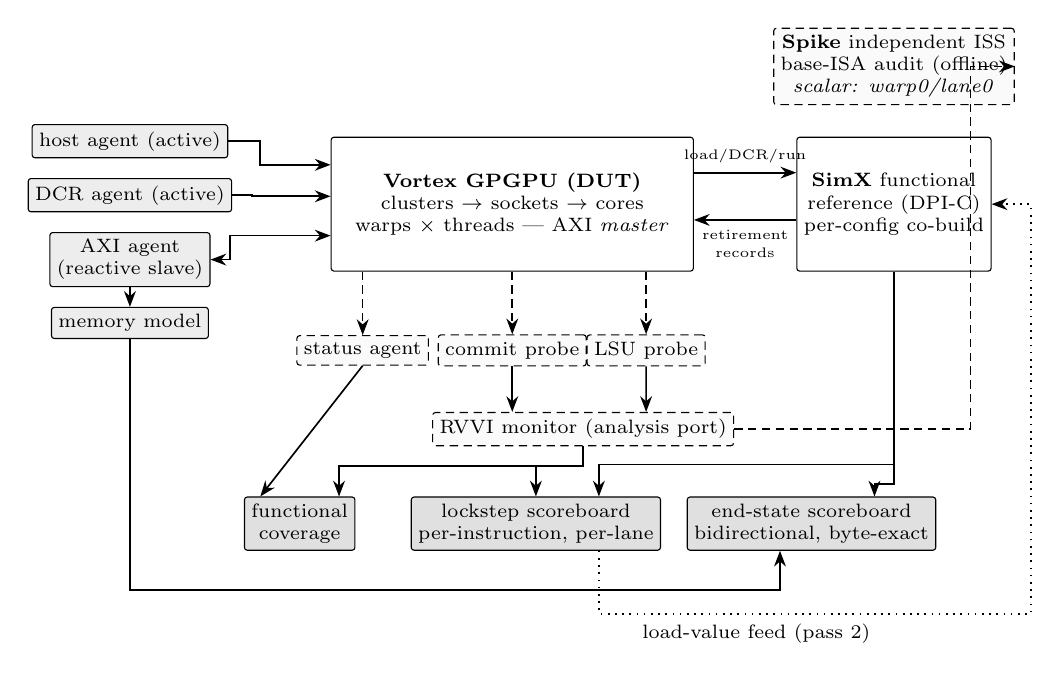
\begin{tikzpicture}[
		font=\scriptsize,
		box/.style={draw, rounded corners=1pt, align=center, inner sep=2.5pt},
		agent/.style={box, fill=gray!14},
		passive/.style={box, fill=gray!4, densely dashed},
		chk/.style={box, fill=gray!24},
		arr/.style={-{Stealth[length=2mm]}, semithick},
		tap/.style={-{Stealth[length=2mm]}, semithick, densely dashed}
		]
		\node[box, minimum width=46mm, minimum height=17mm] (dut)
		{\textbf{Vortex GPGPU (DUT)}\\
			clusters $\to$ sockets $\to$ cores\\
			warps $\times$ threads --- AXI \emph{master}};
		\node[agent, left=13mm of dut.west, anchor=east, yshift=8mm] (host)
		{host agent (active)};
		\node[agent, below=2.5mm of host] (dcr) {DCR agent (active)};
		\node[agent, below=2.5mm of dcr] (axi) {AXI agent\\(reactive slave)};
		\node[agent, below=2.5mm of axi] (mem) {memory model};
		\node[box, right=13mm of dut.east, anchor=west, minimum height=17mm] (simx)
		{\textbf{SimX} functional\\ reference (DPI-C)\\ per-config co-build};
		\node[passive, above=4mm of simx.north, anchor=south, minimum width=30mm] (spike)
		{\textbf{Spike} independent ISS\\ base-ISA audit (offline)\\ \emph{scalar: warp0/lane0}};
		\node[passive] (status) at ($(dut.south)+(-19mm,-10mm)$) {status agent};
		\node[passive] (cprobe) at ($(dut.south)+(0mm,-10mm)$)  {commit probe};
		\node[passive] (lprobe) at ($(dut.south)+(17mm,-10mm)$) {LSU probe};
		\node[passive] (rvvi) at ($(dut.south)+(9mm,-20mm)$)
		{RVVI monitor (analysis port)};
		\node[chk] (cov) at ($(dut.south)+(-27mm,-32mm)$)
		{functional\\ coverage};
		\node[chk] (lss) at ($(dut.south)+(3mm,-32mm)$)
		{lockstep scoreboard\\ per-instruction, per-lane};
		\node[chk] (ess) at ($(dut.south)+(38mm,-32mm)$)
		{end-state scoreboard\\ bidirectional, byte-exact};
		\draw[arr] (host.east) -- ++(4mm,0) |- ([yshift=5mm]dut.west);
		\draw[arr] (dcr.east)  -- ++(2.5mm,0) |- ([yshift=1mm]dut.west);
		\draw[arr, {Stealth[length=2mm]}-{Stealth[length=2mm]}]
		(axi.east) -- ++(2.5mm,0) |- ([yshift=-4mm]dut.west);
		\draw[arr] (axi) -- (mem);
		\draw[arr] ([yshift=4mm]dut.east) -- ([yshift=4mm]simx.west)
		node[midway, above, font=\tiny] {load/DCR/run};
		\draw[arr] ([yshift=-2mm]simx.west) -- ([yshift=-2mm]dut.east)
		node[midway, below, font=\tiny] {\shortstack{retirement\\records}};
		\draw[tap] ([xshift=-19mm]dut.south) -- (status.north);
		\draw[tap] (dut.south) -- (cprobe.north);
		\draw[tap] ([xshift=17mm]dut.south) -- (lprobe.north);
		\draw[arr] (cprobe.south) -- ([xshift=-9mm]rvvi.north);
		\draw[arr] (lprobe.south) -- ([xshift=8mm]rvvi.north);
		\draw[arr] (rvvi.south) -- ++(0,-2.5mm) -| (lss.north);
		\draw[arr] (rvvi.south) -- ++(0,-2.5mm) -| ([xshift=5mm]cov.north);
		\draw[arr] (status.south) -- ([xshift=-5mm]cov.north);
		\draw[arr] (simx.south) -- ++(0,-27mm) -| ([xshift=8mm]ess.north);
		\draw[arr] (simx.south) -- ++(0,-24.5mm) -| ([xshift=8mm]lss.north);
		\draw[arr] (mem.south) |- ($(ess.south)+(-4mm,-5mm)$)
		-- ($(ess.south)+(-4mm,0)$);
		\draw[arr, dotted] ([xshift=8mm]lss.south) -- ++(0,-8mm)
		-| ($(simx.east)+(5mm,0)$) -- (simx.east);
		\node[below] at ($(lss.south)+(28mm,-8mm)$)
		{load-value feed (pass 2)};
		\draw[tap] (rvvi.east) -- ++(30mm,0) |- (spike.east);
	\end{tikzpicture}
	\caption{The environment, in brief. A GPGPU executes programs rather
		than being driven by them, so the UVM roles invert: agents are
		reactive slaves and launchers around a bus-master DUT, stimulus is a
		compiled kernel, and two checkers---a byte-exact bidirectional
		end-state scoreboard and a per-instruction, per-lane lockstep
		comparator---render verdicts against the project's own functional
		simulator (SimX), linked live over DPI.}
	\label{fig:arch}
\end{figure*}

\section{The environment in one figure}
Figure~\ref{fig:arch} shows the shape of the environment. Three
design choices matter for anyone porting the pattern.

\textbf{Roles invert around a GPU.} The DUT is the bus master; UVM
agents are reactive---an AXI responder backed by a memory model
services fetch and data traffic, host and device-configuration agents
drive the launch protocol, and a passive layer of bound probes
(commit arbiter, load-store writeback, scheduler, caches) feeds
checkers and coverage without ever being a checker itself. One
compiled environment runs any cluster/core/warp/thread topology from
plusargs, with elaboration-time assertions cross-checking every
testbench parameter against its DUT counterpart.

\textbf{Verdicts are a taxonomy, and ``unverifiable'' is a
	first-class member.} Every run ends \textsc{pass},
\textsc{fail}, or \textsc{unverifiable}---the last when the golden
model itself cannot judge (say, the reference aborts on an
instruction it cannot decode). Classifying rather than force-fitting
such runs is what preserved our ability to find reference-model bugs
later.

\textbf{Checkers must be proven able to fail.} Each verdict-rendering
checker carries a permanent fault-injection guard in regression:
flip one bit of one store (the end-state scoreboard must catch it),
drop one store (the reverse pass must catch it), corrupt one
retirement (the lockstep must name the exact instruction and lane).
We once nearly accepted a gate whose negative tests reported
\textsc{pass} because their injection plusargs were absent; the
codified rule since then is \emph{verify the injection message, never
	the verdict}. Every number we quote below is backed by checkers that
have been seen to go red.

\section{Lockstep for a warp machine: five rules}
Per-instruction comparison against a functional model is standard for
CPUs~\cite{difftest,imperasdv}; a SIMT GPU breaks the standard in
five specific ways. Each forced a rule, and each rule generalizes to
any warp-based DUT:

\begin{enumerate}
	\item \textbf{Retire order is not program order.} The commit arbiter
	      retires whichever unit is ready; we watched an instruction retire
	      after two later ones. \emph{Align by the per-warp issue counter
		      (uuid), sorted---never by cycle.}
	\item \textbf{The reference has no uuid.} SimX leaves its identifier
	      at zero, so there is no cross-key. \emph{Align both streams by
		      per-(core, warp) program-order position; the DUT's uuid high bits
		      supply the attribution.}
	\item \textbf{One instruction is not one record.} A single load can
	      commit in fragments with overlapping thread masks
	      (\code{0xd} then \code{0xe}) as lanes' memory responses arrive.
	      \emph{Aggregate records by uuid with mask-union before comparing.}
	\item \textbf{Load data is stale at the arbiter and unsafe to compare
		      naively.} Loads of uninitialized memory legitimately differ between
	      models---429 false mismatches on a known-good kernel. \emph{Tap the
		      load-store unit for true values, and compare only where memory state
		      is provably shared; defer the rest to the end-state check.}
	\item \textbf{Performance counters differ by construction.}
	      \code{mcycle} and friends are timing artifacts. \emph{Flag them
		      volatile; compare address and destination, skip the data.}
\end{enumerate}

With the rules in place, the comparator validated lane-exact---zero
mismatches, zero orphans---across five configurations up to two
clusters, two cores, eight warps, including nested-divergence towers
that exercise the mask-union rule through reconvergence. One honest
exception class: the DUT's \code{fsqrt.s} is one ULP off
correctly-rounded IEEE~754, so its writeback is tolerated within one
ULP (tallied, never silent), and a second-pass feed pushes the
accepted result into the reference so the deviation cannot cascade.
That is not a fudge; it is a declared, logged exception---and
Section~\ref{sec:golden} shows what being strict about exceptions
buys you.

\section{Racy programs, verified}
Fenceless multi-core programs have no architecturally defined result:
the two models legitimately resolve the same race differently, and a
per-instruction compare drowns in false mismatches. The standard
responses are to waive such programs or compare only final state. We
do better with a two-pass \emph{load-value feed}: pass one records
the DUT's loaded values at the divergent sites; pass two re-runs the
reference \emph{following} those values, so both models share each
race outcome---and any remaining difference is a real defect. On the
flagship case, twenty racy loads cascading into 138 divergent
retirements collapse to a residual of \textbf{zero over 5{,}432
	retirements}.

The soundness assumption is stated, not smuggled: the feed is honest
exactly when a divergent load is a genuine race resolution rather
than a load-data bug. In the flagship case we confirmed it by
trace---the loaded word still held its pristine initialization value,
proving a cross-core ordering race. Where the fixed point genuinely
does not exist, we say so: asynchronous interrupts (the models take
them at different instruction boundaries) and races that steer
control flow remain unverified at instruction granularity, classified
rather than forced green.

\section{The headline lesson: audit the golden model too}
\label{sec:golden}
A lockstep flow compares two artifacts, and only one of them is the
RTL. SimX is maintained by the same project as the DUT---and our
per-instruction compare found it defective, more than once.

The reference fetched instructions at the exact byte program counter.
A computed jump to an odd target---which the RTL tolerates by
word-aligning---made SimX read across an instruction boundary and
abort, silently discarding verification results as ``unverifiable''
runs. The lockstep's own divergence report localized the bug.
Tellingly, the obvious fix---masking the jump target in the
model---made things \emph{worse}: 21{,}968 phantom mismatches,
because it corrected the model toward the specification instead of
toward the DUT. A golden model's job is to mirror the design as
built; where design and specification disagree, that disagreement is
a finding, not something to launder.

Then came the symmetric exchange with the fuzzing world. We ran
FuzzGPU's reported Vortex bugs at our pin. One reproduced as an RTL
defect (an FPU writeback rule violation, firing the RTL's own
assertion). The second---publicly described as a hardware bug and
fixed upstream as such---reproduced as a divergence in which
\emph{the hardware was right and the golden model was wrong}: the
upstream fix lives entirely in the simulator's decoder. Only a
DUT-versus-reference comparison could attribute that correctly. Two
methodologies, two directions of mislabeling, both caught: their
``hardware bug'' was our golden-model bug, and our hardware's ISA
deviation (JALR not clearing the target LSB, with real architectural
consequences) had been independently found by their fuzzing. If you
run lockstep against a project-internal model, budget for verifying
the model---it will need it.

\section{Coverage you can defend}
Functional coverage for a GPU needs a layer that does not exist
anywhere in the scalar world: SIMT microarchitecture coverage. Our
model adds warp-divergence depth crossed with the reconvergence
stack, scratchpad bank conflicts, and memory-coalescing
classes---to our knowledge the first published such layer---atop a
third-party ISA layer and a protocol layer. Closure on the primary
configuration reached 98.1\% of covergroup bins (94.7\% total), with
the ISA layer separately at 83.1\% of bins. Full provenance,
configuration by configuration, is in our preprint~\cite{preprint}.

Three disciplines make those numbers defensible rather than
decorative:

\textbf{Exclusions are machine-generated and gate-checked.} Every
waiver cites RTL \code{file:line}; a blocking ``hits-invariant''
check aborts any merge in which a waived bin had actually been hit.
That gate has caught three classes of defect in operation, including
its own operator: an exclusion set generated with the wrong
configuration's keys aborted a merge that would otherwise have
silently corrupted a 110-run bank. A methodology whose bookkeeping
catches its operator's mistakes is the minimum bar for trusting a
signed-off percentage.

\textbf{Coverage definitions are verification targets too.} Our bank
-conflict coverpoint, defined over \emph{accepted} requests, could
never hit---the crossbar admits one winner per bank per cycle. The
``stimulus gap'' was a definition defect; deliberate bank-hostile
stimulus proved it by producing zero conflicts, and redefining the
coverpoint over \emph{offered} requests made it reachable and honest.
Validate the coverage model against the RTL, not just the RTL against
the model.

\textbf{Negative results are results.} Ninety additional
random programs from a scalar generator closed \emph{zero} coverage
bins---every category bit-identical. Coverage saturates inside a
stimulus kind; more seeds of the same kind buy nothing. Only
SIMT-aware generated kernels closed the SIMT-specific targets
(divergence depth, bank conflicts). Kind, not volume, moves a mature
coverage model.

\section{What does it cost?}
Measured on four kernels across three modes---plain environment,
lockstep on, lockstep plus the two-pass feed---the answer is: far
less than the value of what it catches (Table~\ref{tab:cost}).
Lockstep adds no measurable wall-clock overhead at any kernel size;
its real cost is memory, roughly 29\% peak RSS at the largest working
set for the second model instance. The feed is free. One accident
was instructive: the FPU kernel under plain lockstep fails exactly as
the fsqrt exception-class design predicts, and passes with the feed
armed---the cheapest possible demonstration that the exception
machinery does what its documentation says.

\begin{table}[t]
	\caption{What the checking stack costs (medians; QuestaSim).}
	\label{tab:cost}
	\centering
	\small
	\begin{tabular}{llcc}
		\toprule
		Kernel         & Mode     & Wall    & Peak RSS \\
		\midrule
		small baseline & plain    & 15.3\,s & 296\,MB  \\
		               & lockstep & 15.0\,s & 299\,MB  \\
		               & +feed    & 14.8\,s & 299\,MB  \\
		large memory   & plain    & 851\,s  & 549\,MB  \\
		               & lockstep & 871\,s  & 708\,MB  \\
		               & +feed    & 856\,s  & 708\,MB  \\
		\bottomrule
	\end{tabular}
\end{table}

\section{What the checking found}
Beyond the reset relay and the golden-model defects: the JALR LSB
deviation (independently corroborated by FuzzGPU, and later found by
us to cascade into silent misaligned accesses through
address-generation instructions); a watchdog constant written as
\code{1**N}---one, for any N---that disabled stall detection at every
scale, independently fixed upstream after we reported it; a
fire-and-forget AXI write path with no error response handling,
proven by injecting \code{SLVERR} on every seventh transaction (166
firings, no recovery); a \code{fsqrt.s} one ULP off correctly
rounded, invisible to any end-state tolerance and caught only by
per-instruction compare; and a memory-scheduler timeout denominated
in picoseconds that floods L2/L3 runs with tens of thousands of
false alarms. The full register---sixty-plus entries, each with
evidence and a disposition---ships with the artifact~\cite{preprint}.

\section{Takeaways}
\begin{itemize}
	\item \textbf{A silenced checker is a deaf checker.} Guards added to
	      make bring-up survivable must be tracked and re-litigated; the
	      assertion we restored had been right all along, and its message had
	      been the only witness to a real defect.
	\item \textbf{Expect coverage to move \emph{down} when you fix
		      certain bugs.} If it does not, you may be counting coverage earned in
	      illegitimate states.
	\item \textbf{Lockstep verifies two artifacts.} Treat the golden
	      model as a verification target, or it will quietly misattribute
	      findings---possibly at a security conference's expense.
	\item \textbf{Gate your waivers.} An exclusion that cannot prove it
	      excluded nothing real is a liability.
	\item \textbf{Stimulus kind beats stimulus volume.} Buy generators
	      that target what your coverage model says is missing, not more seeds
	      of what it already has.
	\item \textbf{The GPU is not a big CPU.} Inverted agent roles, split
	      retirements, and divergence-aware alignment are the price of
	      admission---and, once paid, everything else transfers.
\end{itemize}

\section{Conclusion}
Open hardware now includes processors complex enough to deserve
industrial verification, and attackers have noticed. We built that
verification for Vortex---lockstep, racy-program checking, and a
SIMT coverage model---and the exercise taught the harder lesson:
the discipline you impose on the design must be imposed on every
artifact in the loop, including the reference model and the coverage
model itself. The environment, the evidence registers, and every
number's provenance are open~\cite{preprint}. The boulder rolls; so
does the regression.

\section*{Acknowledgment}
The authors thank the Vortex group at Georgia Tech and the
maintainers of core-v-verif, riscv-dv, RVVI, riscvISACOV, and Spike.

\begin{thebibliography}{15}
	\bibitem{vortex-micro}
	B.~Tine, K.~P. Yalamarthy, F.~Elsabbagh, and H.~Kim, ``Vortex:
	Extending the RISC-V ISA for GPGPU and 3D-graphics,'' in \emph{Proc.
		MICRO-54}, 2021, pp. 754--766.
	\bibitem{fuzzgpu}
	Z.~Gao \emph{et al.}, ``Fuzzing open-source GPU hardware with SIMT
	program generation,'' in \emph{Proc. 35th USENIX Security Symp.},
	2026, pp. 2465--2484.
	\bibitem{corevverif}
	OpenHW Group, ``core-v-verif.'' [Online]. Available:
	\url{https://github.com/openhwgroup/core-v-verif}
	\bibitem{riscvdv}
	CHIPS Alliance, ``riscv-dv.'' [Online]. Available:
	\url{https://github.com/chipsalliance/riscv-dv}
	\bibitem{rvvi}
	OpenHW Group / Imperas, ``RISC-V Verification Interface.'' [Online].
	Available: \url{https://github.com/riscv-verification/RVVI}
	\bibitem{imperasdv}
	Imperas Software, ``ImperasDV.'' [Online]. Available:
	\url{https://imperas.com/imperasdv}
	\bibitem{opentitan}
	lowRISC, ``OpenTitan.'' [Online]. Available:
	\url{https://github.com/lowRISC/opentitan}
	\bibitem{difftest}
	Y.~Xu \emph{et al.}, ``Towards developing high-performance RISC-V
	processors using agile methodology,'' in \emph{Proc. MICRO-55}, 2022.
	\bibitem{gpuverify}
	A.~Betts, N.~Chong, A.~F. Donaldson, S.~Qadeer, and P.~Thomson,
	``The design and implementation of a verification technique for GPU
	kernels,'' \emph{ACM TOPLAS}, vol. 37, no. 3, 2015.
	\bibitem{gklee}
	G.~Li \emph{et al.}, ``GKLEE: Concolic verification and test
	generation for GPUs,'' in \emph{Proc. PPoPP}, 2012, pp. 215--224.
	\bibitem{vacuity-date10}
	L.~Di Guglielmo, F.~Fummi, and G.~Pravadelli, ``Vacuity analysis for
	property qualification by mutation of checkers,'' in \emph{Proc.
		DATE}, 2010, pp. 262--267.
	\bibitem{nvbitfi}
	T.-T.~Tsai \emph{et al.}, ``NVBitFI: Dynamic fault injection
	methodology for GPU applications,'' in \emph{Proc. DSN}, 2021,
	pp. 64--76.
	\bibitem{preprint}
	S.~Moussa \emph{et al.}, ``SIMT-aware lockstep verification and
	functional-coverage closure methodology for an open-source RISC-V
	GPGPU: a UVM 1.2 environment,'' arXiv preprint (cs.AR), 2026.
	\bibitem{uvm}
	\emph{IEEE Standard for UVM Language Reference Manual}, IEEE Std
	1800.2-2020, 2020.
	\bibitem{rtlcheck}
	Y.~A. Manerkar \emph{et al.}, ``RTLCheck: A property checking
	approach for custom memory consistency models,'' in \emph{Proc.
		MICRO-50}, 2017, pp. 713--725.
\end{thebibliography}

\end{document}
